การออกแบบทางโครงสร้างทางกลของหุ่นยนต์ฮิวมานอยด์ UTHAI นั้น ผู้วิจัยได้เลือกใช้โปรแกรมออกแบบโครงสร้างเป็นโปรแกรม Solidworks
ที่ช่วยในการพัฒนาแบบจำลองของหุ่นยนต์ฮิวมานอยด์ UTHAI
เนื่องจากโปรแกรม Solidworks เป็นโปรแกรมที่ใช้ในการออกแบบ และวาดแบบทางวิศวกรรม
สามารถวิเคราะห์โครงสร้างการรับแรงของแบบจำลองได้ อีกทั้งยังเป็นเครื่องมือที่มีการใช้งานอย่างแพร่หลาย
ทำให้สามารถดาวน์โหลดแบบจำลองต่างๆที่มีคนพัฒนาเข้าเข้ามาใช้ร่วมกับการออกแบบได้ 
และด้วยทางผู้วิจัยมีความคำนึงถึงการพัฒนา ต่อยอดเป็นหลัก ดังนั้นการออกโครงสร้างทางกลของหุ่นยนต์ฮิวมานอยด์ UTHAI
จึงถูกออกแบบมาเพื่อให้สามารถรองรับการปรับเปลี่ยน เปลี่ยนแปลง แก้ไขชิ้นส่วนต่างๆของตัวหุ่นยนต์ฮิวมานอยด์ UTHAI ต่อไปได้

\subsection{โครงสร้างหุ่นยนต์}
หุ่นยนต์ฮิวมานอยด์ที่สร้างขึ้นประกอบด้วยส่วนของลำตัวและส่วนขา ในขาแต่ละข้างออกแบบให้ข้อต่อมีเป็นลักษณะของข้อต่อแบบหมุน (Revolute joint)
เพื่อเลียนแบบโครงสร้างของมนุษย์ที่ประกอบด้วย ส่วนของสะโพกที่มีองศาอิสระจำนวน 3 องศาอิสระ หัวเข่า 1
องศาอิสระ และข้อเท้า 2 องศาอิสระ รวมทั้งขาข้างละ 6 องศาอิสระ ระบบต้นกำลังที่ใช้ในแต่ละข้อต่อเป็นดิจิตอลเซอร์โว
การออกแบบหุ่นยนต์ฮิวมานอยด์ UTHAI นั้น
สิ่งแรกที่ต้องทำ คือ การกำหนดโครงสร้างของข้อต่อและก้านต่อ ดังรูปที่ \ref{fig:uthai_design_structure}
ซึ่งโครงสร้างนั้นทางผู้วิจัยได้อ้างอิงมาจากสัดส่วนของมนุษย์จริง
และมีจุดศูนย์กลางมวลอยู่บริเวณกระดูกเชิงกรานของตัวหุ่นยนต์ฮิวมานอยด์เอง ดังรูปที่ \ref{fig:uthai_structure1}

\begin{figure}[!ht]
    \centering
    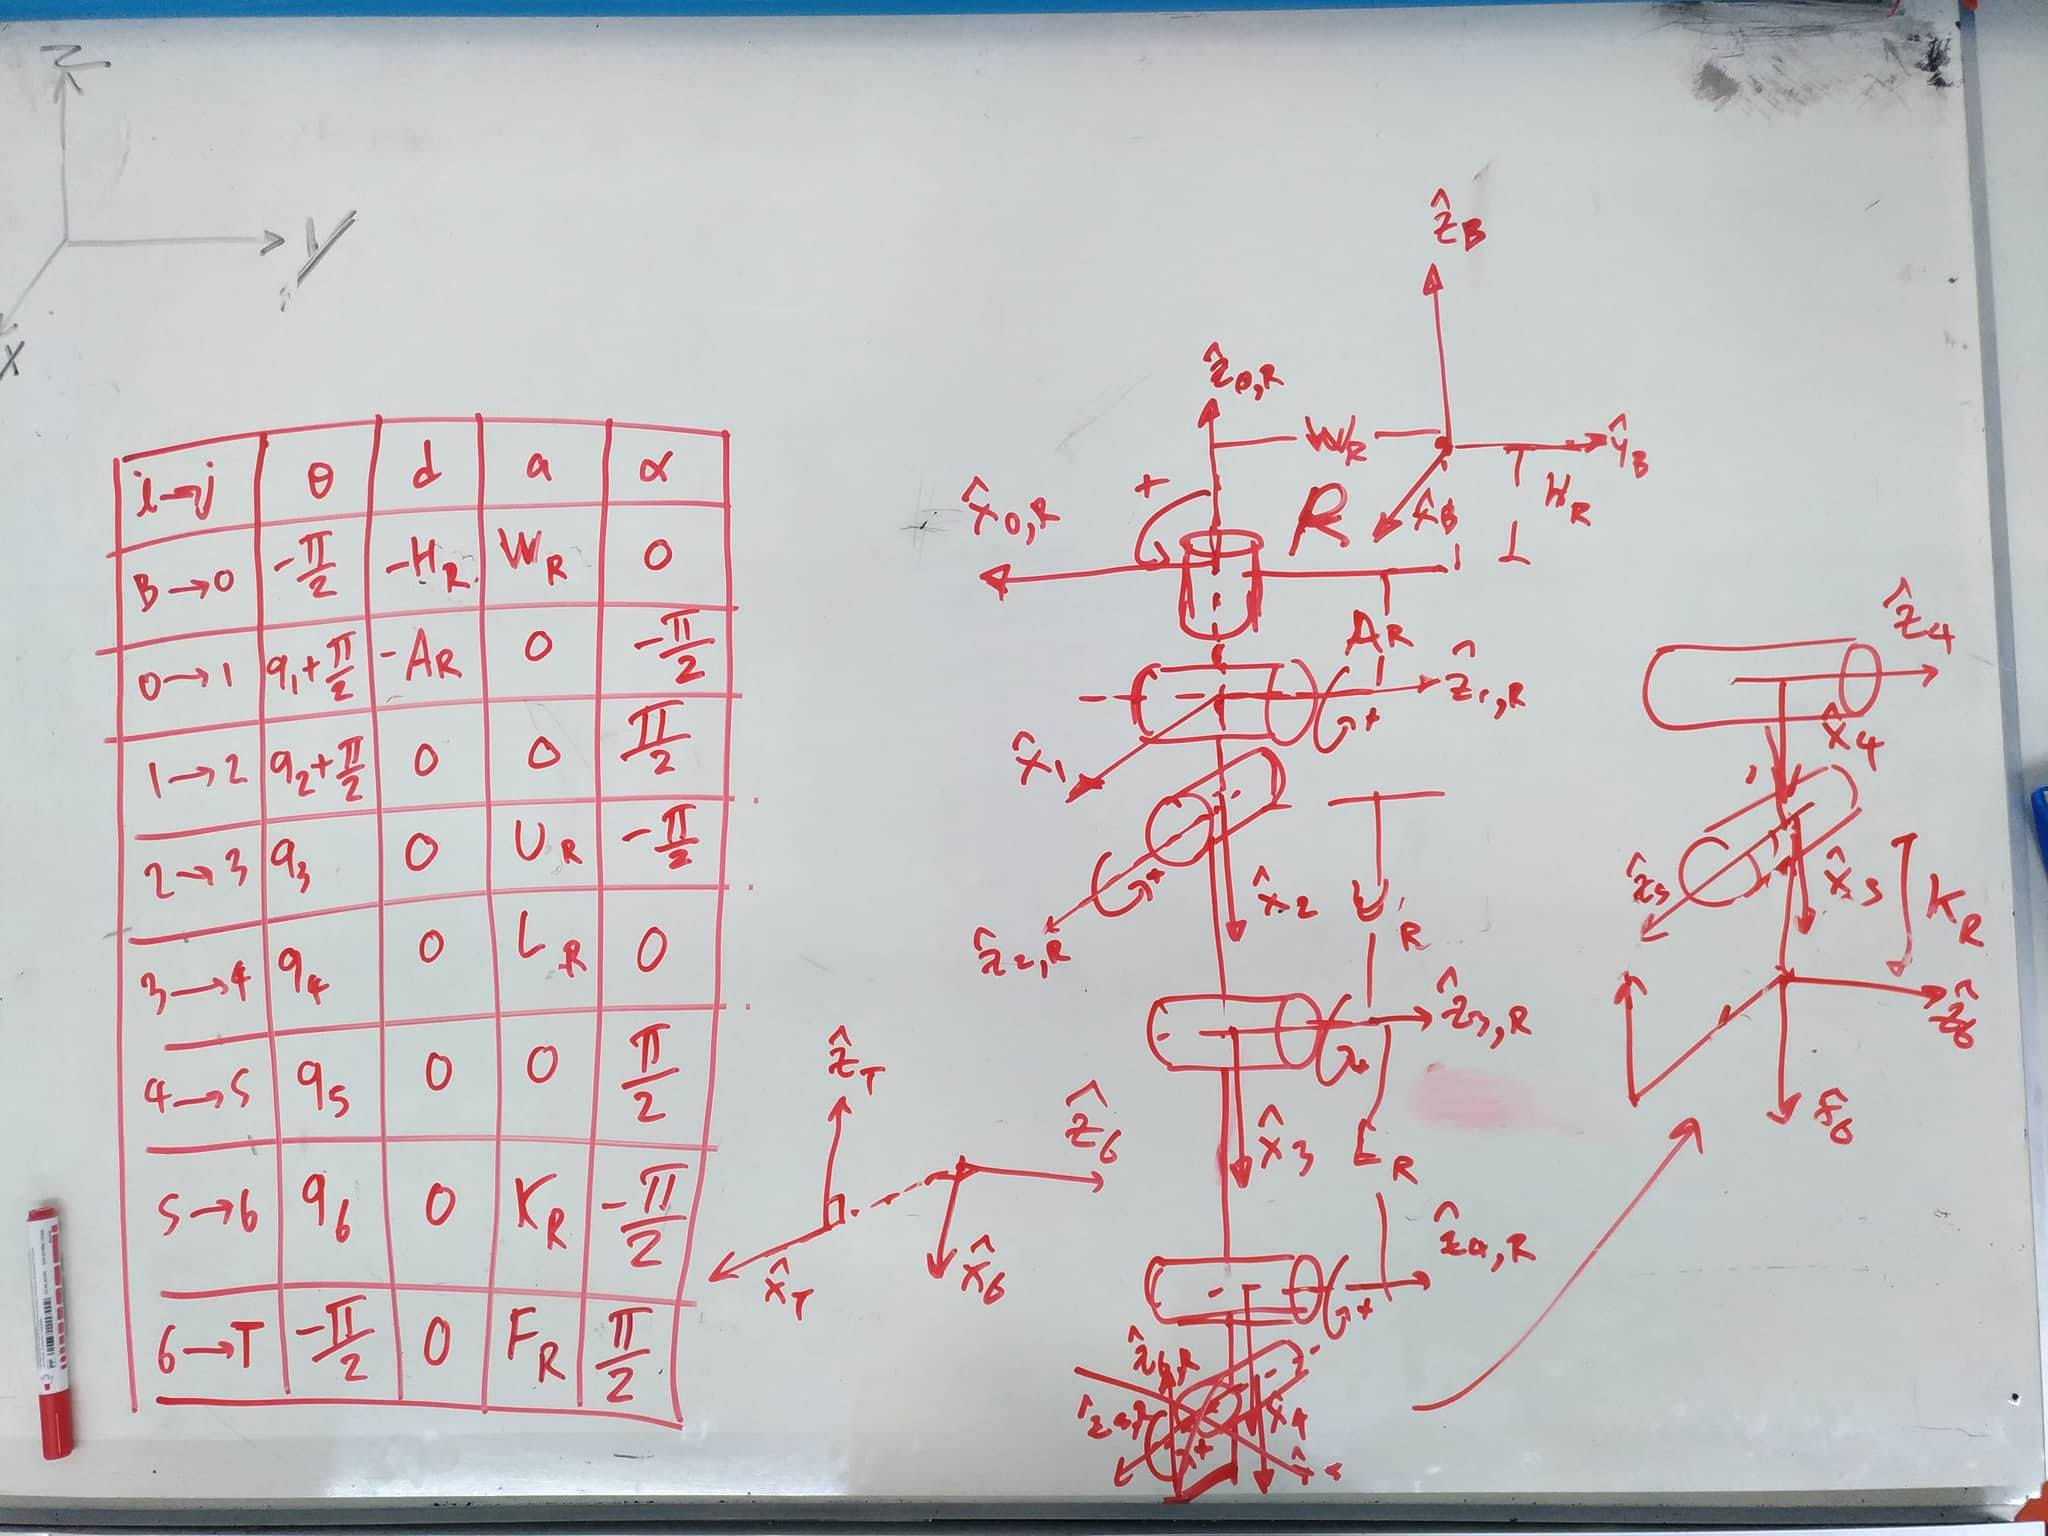
\includegraphics[width=0.5\textwidth]{chapter3/images/clean/uthai_design_structure.jpg}
    \caption{การออกแบบโครงสร้างของหุ่นยนต์ UTHAI}
    \label{fig:uthai_design_structure}
\end{figure}

\begin{figure}[!ht]
    \centering
    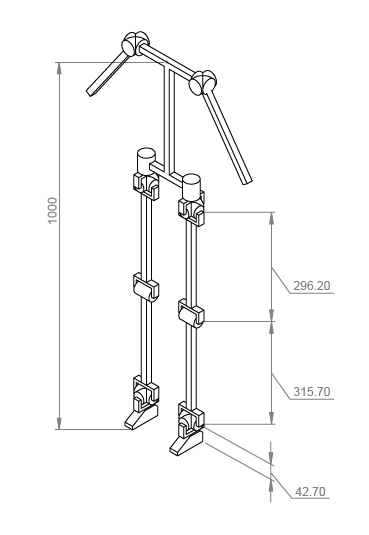
\includegraphics[width=0.35\textwidth]{chapter3/images/uthai_structure1.png}
    \caption{ภาพแสดงแสดงโครงสร้างของหุ่นยนต์ UTHAI}
    \label{fig:uthai_structure1}
\end{figure}

เมื่อเราได้แบบของหุ่นยนต์ฮิวมานอยด์ UTHAI แล้ว ลำดับต่อไปคือการกำหนดตำแหน่งการติดตั้งเซนเซอร์และตัวขับเคลื่อนต่างๆเข้าไป
โดยมีเซนเซอร์ตรวจการสัมผัสพื้นติดตั้งที่ใต้ฝ่าเท้าของหุ่นยนต์ เซนเซอร์หน่วยวัดความเฉื่อยติดตั้งไว้บริเวณลำตัวของหุ่นยนต์ฮิวมานอยด์
และที่ข้อต่อในแต่ละจุดใช้ตัวขับเคลื่อนเป็นดิจิตอลเซอร์โว ดังรูปที่ \ref{fig:uthai_structure2}

\begin{figure}[!ht]
    \centering
    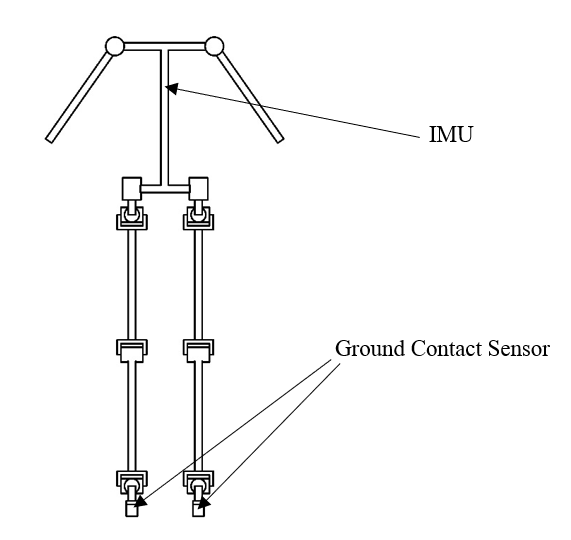
\includegraphics[width=0.5\textwidth]{chapter3/images/uthai_sensor.PNG}
    \caption{ภาพแสดงการติดตั้งเซนเซอร์ในจุดต่างๆ}
    \label{fig:uthai_structure2}
\end{figure}

ส่วนวัสดุที่ใช้ทำโครงสร้างหุ่นยนต์ฮิวมานอยด์ UTHAI ทางผู้วิจัยเลือกใช้วัสดุหลักเป็น PLA ที่ขึ้นรูปด้วยวิธีการขึ้นรูปสามมิติ
ก้านต่อเป็นคาร์บอนไฟเบอร์ เนื่องจากจะทำให้โครงสร้างมีน้ำหนักเบา ขึ้นรูปได้สะดวกทำให้สามารถปรับปรุงแก้ไขง่าย
และมีวัสดุเสริมบางชิ้นส่วนที่ทำจากอลูมิเนียมเนื่องจากต้องการความแข็งแรงมาก ดังตารางที่ \ref{tab:material_properties}

\begin{table}[!ht]
	\centering
	\begin{tabular}{| l | l | l |}
		\hline
		Material & Longitudinal Tensile Strength ($ksi$) & Density ($g/cm^3$) \\
        \hline
        Carbon Fiber & 300 & 1.55 \\
        Steel & 100	& 7.7 \\
        Titanium & 120 & 4.34 \\
        Aluminum & 35 & 2.7 \\
        PLA 3D printing (50 \% infill) & 3.5 & 1.26 \\
        PLA 3D printing (100 \% infill) & 5.5 & 1.26 \\
	    \hline
	\end{tabular}
	\caption{ตารางแสดงสมบัติทางกลของวัสดุต่าง ๆ}
	\label{tab:material_properties}
\end{table}

\clearpage
\subsection{จัดทำชิ้นส่วนโครงสร้าง}
ในกาารจัดทำชิ้นส่วนโครงสร้างของหุ่นยนต์ฮิวมานอยด์อุทัยนั้นทาง ผู้วิจัยได้คำนึงถึงความแข็งแรงเป็นหลักซึ่งมีความสำคัญมาก
ในการเคลื่อนที่ของหุ่นยนต์ อีกทั้งยังต้องมีน้ำหนักที่เบาเพื่อประหยัดพลังงานที่ต้องใช้ในการขับเคลื่อน\footnote{ Printing Guide [https://filaments.ca/pages/temperature-guide]}
ดังนั้นผู้วิจัยจึงได้ใช้การขึ้นรูปชิ้นงานด้วยเทคนิคการพิมพ์สามมิติ โดยจะใช้วัสดุหลักเป็นพลาสติก PLA ซึ่งมีความแข็งมากกว่าและขึ้นรูปง่ายกว่าพลาสติกชนิด ABS ดังตารางที่ \ref{tab:plastic_material_properties}
และก้านต่อเป็นคาร์บอนไฟเบอร์ เพื่อให้ตอบโจทย์กับหุ่นยนต์แพลตฟอร์มเพื่อพัฒนาต่อยอดในอนาคต
ซึ่งผู้ใช้ทุกคนสามารถพิมพ์ชิ้นงานขึ้นมาได้ด้วยตนเอง\footnote{ PLA vs ABS [https://www.3dhubs.com/knowledge-base/pla-vs-abs-whats-difference]}

\begin{table}[!ht]
	\centering
	\begin{tabular}{| l | l | l |}
		\hline
		Properties & ABS & PLA \\
        \hline
        Tensile Strength & 27 $MPa$ & 37 $MPa$ \\
        Elongation & 3.5 \- 50\% & 6\% \\
        Flexural Modulus & 2.1 \- 7.6 $GPa$ & 4 $GPa$ \\
        Density & 1.0 - 1.4 $g/cm^3$ & 1.3 $g/cm^3$ \\
        Melting Point & 230$°C$ - 240$°C$ & 215$°C$ - 235$°C$ \\ 
        การย่อยสลายทางธรรมชาติ & ไม่ได้ & ได้ (ภายใต้เงื่อนไขที่ถูกต้อง) \\
	    \hline
	\end{tabular}
	\caption{ตารางแสดงสมบัติทางกลของวัสดุพลาสติก}
	\label{tab:plastic_material_properties}
\end{table}

แต่เนื่องจากในปัจจุบันนี้เครื่องพิมพ์สามมิติส่วนมากจะไม่รองรับการพิมพ์ชิ้นงานที่มีขนาดใหญ่ ซึ่งมีขนาดมากกว่า
30x30x30 ซม. (กว้างxยาวxสูง) ดังนั้นชิ้นงานที่ขึ้นรูป ที่มีขนาดใหญ่เกินกว่านี้อาจจะต้องทำการตัดชิ้นงานออกเป็นส่วนย่อยๆก่อน
แล้วจึงค่อยนำมาประกอบรวมกันทีหลังอีกครั้งหนึ่ง โดยพื้นที่ทำการพิมพ์ของเครื่องพิมพ์สามมิติที่มีวางจำหน่าย\footnote{The truth about 3D printer maximum print areas [https://www.zdnet.com/article/what-manufacturers-dont-want-you-to-know-the-truth-about-3d-printer-maximum-print-areas/]}
และใช้งานแพร่หลายในท้องตลาดแสดง ดังตารางที่ \ref{tab:3dprint_space} 
\begin{table}[!ht]
	\centering
	\begin{tabular}{| l | l | l | l |}
		\hline
		ชื่อเครื่องพิมพ์สามมิติ & ขนาดความกว้าง (มม.) & ขนาดความลึก (มม.) & ขนาดความสูง (มม.) \\
        \hline
        MakerBot Replicator+ & 292 & 192 & 165 \\
        Ultimaker 3 & 188 & 185 & 200 \\
        LulzBot Mini & 152 & 152 & 158 \\
        Dreammaker Overlord Pro Plus & 79 & 79 & 255 \\
        New Matter MOD-t & 145 & 95 & 125 \\
	    \hline
	\end{tabular}
	\caption{ตารางแสดงขนาดของชิ้นงานที่สามารถพิมพ์ได้ในเครื่องพิมพ์ชนิดต่างๆ}
	\label{tab:3dprint_space}
\end{table}



%%%%%%%%%%%%%%%%%%%%%%%%%%%%%%%%%%%%%%%%%%%%%%%%%%%%%%%%%%%%%%%%%%%%%%%%%%%%%%%
%%%%%%%%%%%%%%%%%%%%%%%%%%%%%%%%%%%%%%%%%%%%%%%%%%%%%%%%%%%%%%%%%%%%%%%%%%%%%%%
%%%%%%%%%%%%%%%%%%%%%%%%%%%%%%%%%%%%%%%%%%%%%%%%%%%%%%%%%%%%%%%%%%%%%%%%%%%%%%%
\clearpage
\subsection{อุปกรณ์ที่ใช้ในหุ่นยนต์ฮิวมานอยด์ UTHAI}

\subsubsection*{Dynamixel Servo EX-106+}
Dynamixel EX-106+ เป็นตัวขับเคลื่อนที่นิยมใช้ในหุ่นยนต์ปัจจุบัน ซึ่งเป็นเซอร์โวมอเตอร์ที่เหมาะสำหรับทำหุ่นยนต์โดยเฉพาะ
ภายในประกอบไปด้วย มอเตอร์กระแสตรง ชุดเฟืองมอเตอร์ ไดรเวอร์คอนโทรเลอร์ สามารถเชื่อมต่อกันผ่านบัส RS-485
\footnote{ Robot Actuator [http://support.robotis.com/en/product/actuator/dynamixel/ex\_series/ex-106.htm] }
มีการควบคุมตำแหน่งและความเร็วด้วย PID ภายในมีเซนเซอร์สามารถที่จะอ่านค่าความเร็ว
แรงดันไฟฟ้า กระแสไฟฟ้า อุณหภูมิ ตำแหน่ง และแรงบิดจากมอเตอร์ทุกตัวได้ แต่ละมอเตอร์แต่ละตัวจะมีบอร์ดควบคุมของตัวเอง
เราสามารถที่จะจ่ายไฟให้มอเตอร์และควบคุมผ่าน Serial ได้ ดังรูปที่ \ref{fig:dxl_ex106}
การทำงานของตัวดิจิตอลเซอร์โวนี้สามารถทำได้ 2 รูปแบบ\footnote{ EX-106+ Mode [http://www.trossenrobotics.com/dynamixel-ex-106-robot-actuator.aspx]}
คือ

\paragraph*{Joint Mode}
สามารถที่จะควบคุมแรงบิด ความเร็ว และตำแหน่งได้ ความละเอียดในการควบคุมตำแหน่งอยู่ที่ 10bit (0-1023) หมุนได้อยู่ในช่วง -150 ถึง 150 องศา

\paragraph*{Wheel Mode}
สามารถที่จะควบคุมแรงบิด ความเร็ว และทิศทางได้ ความละเอียดของความเร็วอยู่ที่ 10bit (0-1023) สามารถหมุนได้ครบ 360 องศาได้ ความเร็วสูงสุดอยู่ที่ 114 RPM

\begin{figure}[!ht]
    \centering
    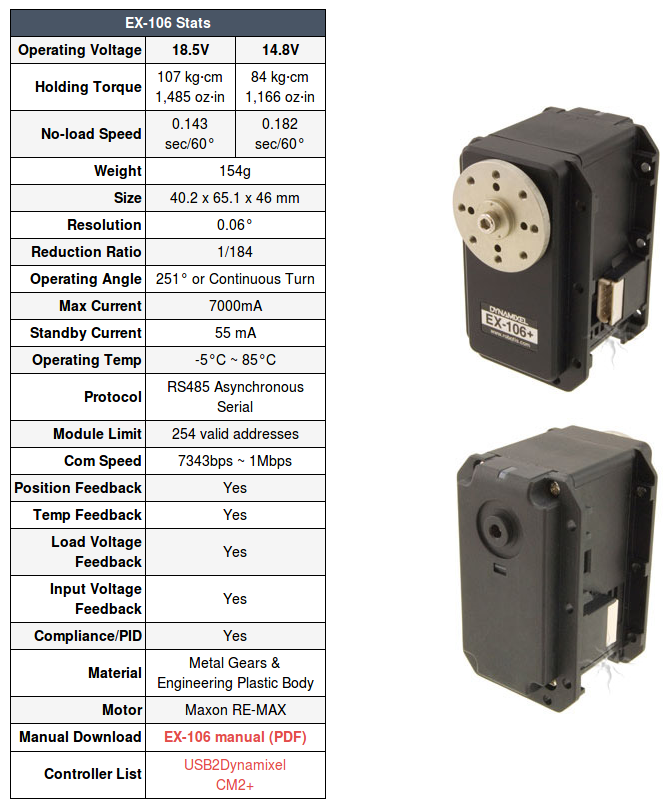
\includegraphics[width=0.7\textwidth]{chapter3/images/dxl_ex106.png}
    \caption{แสดงประสิทธิภาพของมอเตอร์ EX-106+}
    \label{fig:dxl_ex106}
\end{figure}


\clearpage
\subsubsection*{USB2Dynamixel}
USB2Dynamixel เป็นอุปกรณ์สำหรับเชื่อมต่อดิจิตอลเซอร์โว กับหน่วยประมวลผลระดับสูง (Odroid) โดยจะเชื่อมต่อผ่านพอร์ท USB
ที่อยู่บน Odroid และแปลงให้ส่งข้อมูลไปยังดิจิตอลเซอร์โวผ่านสาย 2 เส้น คือ D+ และ D- ดังรูปที่ \ref{fig:dynamixel2pc}
เป็นการเชื่อมต่อแบบ RS-485\footnote{USB2Dynamixel [http://support.robotis.com/en/product/auxdevice/interface/usb2dxl\_manual.html]}
ืทำให้สามารถส่งข้อมูลไปยังหลายๆอุปกรณ์บนสายเส้นเดียวได้
และสามารถส่งในระยะทางไกลๆได้\footnote{http://support.robotis.com/en/images/product/auxdevice/interface/}


\begin{figure}[!ht]
    \centering
    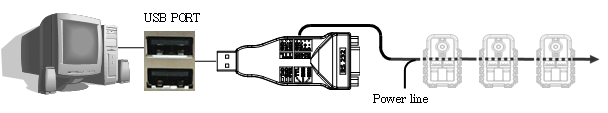
\includegraphics[width=0.75\textwidth]{chapter3/images/dynamixel2pc.png}
    \caption{ภาพแสดงการติดต่อสื่อสารระหว่างคอมพิวเตอร์กับดิจิตอลเซอร์โว}
    \label{fig:dynamixel2pc}
\end{figure}

ในการใช้งาน ผู้ใช้งานจำเป็นต้องเลือกรูปแบบการติดต่อสื่อสารซึ่งแต่ละรูปแบบก็จะมีลักษณะการเชื่อมต่อที่แตกต่างกันไป
USB2Dynamixel ได้แบ่งการติดต่อสื่อสารออกเป็น 3 รูปแบบ\footnote{http://support.robotis.com/en/product/auxdevice/interface/usb2dxl\_manual.htm}คือ
ดังรูปที่ \ref{fig:useusb2dynamixel}
\vspace{-10pt}
\begin{enumerate}[label=\arabic*, leftmargin=1.5cm]
    \setlength\itemsep{-0.25em}
    \item TTL Communication : สำหรับดิจิตอลเซอร์โวที่ใช้พอร์ทชนิด 3-pin ในตระกูล AX Series
    \item RS485 Communication : สำหรับดิจิตอลเซอร์โวที่ใช้พอร์ทชนิด 4-pin ในตระกูล DX Series
    \item RS232 Communication : ใช้สำหรับติดต่อสื่อสารกับคอนโทรลเลอร์ผ่านสายเคเบิล
\end{enumerate}
\vspace{-15pt}
\begin{figure}[!ht]
    \centering
    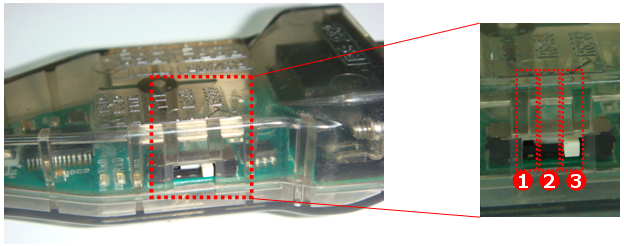
\includegraphics[width=0.5\textwidth]{chapter3/images/useusb2dynamixel.png}
    \caption{ภาพแสดงการเลือกโหมดใช้งานของ USB2Dynamixel}
    \label{fig:useusb2dynamixel}
\end{figure}

แต่จากการทดลองนำมาใช้ ผู้วิจัยพบว่าดิจิตอลที่ใช้ในการทำงานวิจัยครั้งนี้เป็นชนิด 4-pin ซึ่งใช้ RS485 ในการติดต่อสื่อสาร
ด้วยขนาดของตัว USB2Dynamixel มีขนาดที่ใหญ่ทำให้การทำงานมีความลำบากในการติดตั้งลงบนตัวของหุ่นยนต์ฮิวมานอยด์อุทัย
จึงได้ทำการเปลี่ยนเป็น USB2RS485\footnote{https://softgenie.dk/diverse/280-usb2rs485.html}
\begin{figure}[!ht]
    \centering
    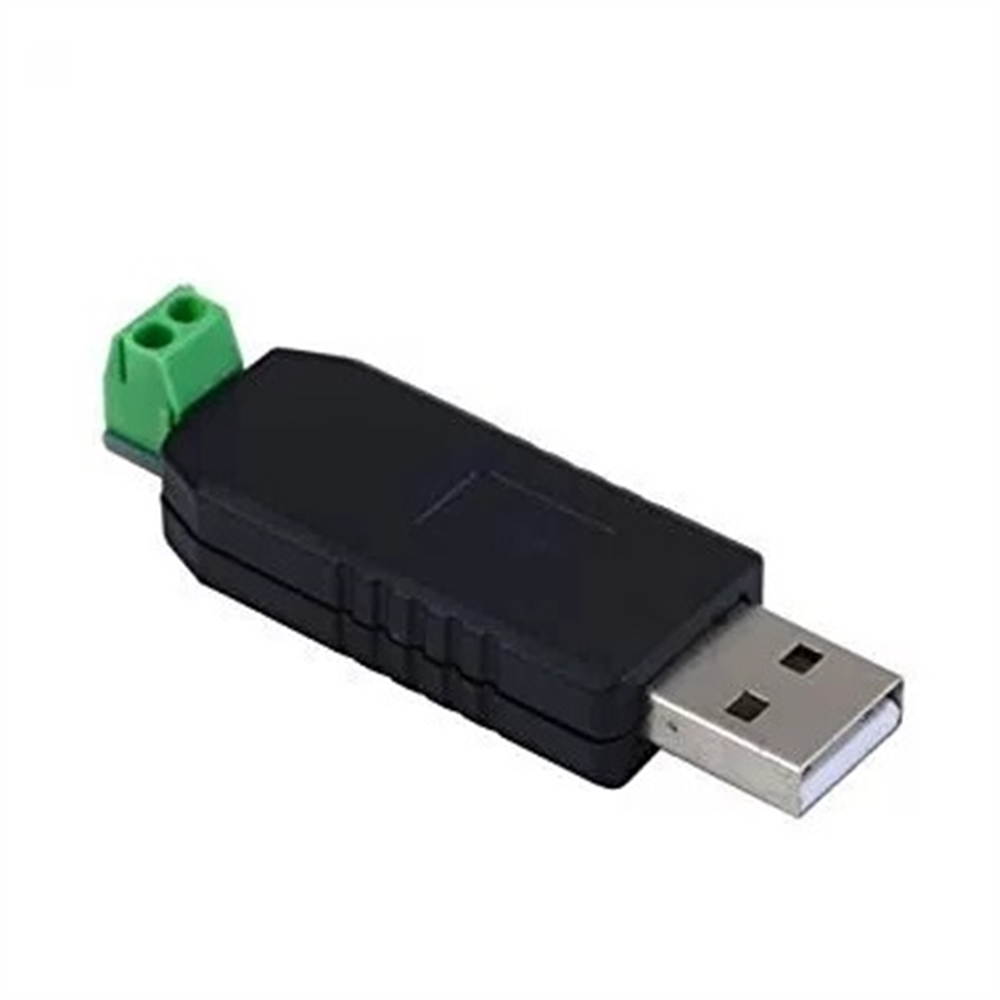
\includegraphics[width=0.25\textwidth]{chapter3/images/usb2rs485.jpg}
    \caption{USB2RS485 Module}
    \label{fig:usb2rs485}
\end{figure}

\clearpage
\subsubsection*{Inertial Measurement Unit (IMU)}
ผู้วิจัยได้เลือกใช้เซนเซอร์หน่วยวัดความเฉื่อยเป็น MPU-9250 ดังรูปที่ \ref{fig:mpu9250} มาใช้ในการอ่านหาค่ามุมเอียงของฐานหุ่นยนต์ฮิวมานอยด์อุทัย
เพื่อใช้ในการคุมเสถียรภาพของหุ่นยนต์
โดยเซนเซอร์ตัวนี้สามารถวัดค่าได้ 9 แกนคือ วัดค่าความเร็วเชิงมุม (gyroscope) 3 แกน วัดค่าความเร่งเชิงเส้น (accelerometer) 3 แกน
และวัดค่าสนามแม่เหล็กโลก (magnetometer) 3 แกน ซึ่งเซนเซอร์จะติดตั้งบริเวณส่วนของลำตัวหุ่นยนต์ฮิวมานอยด์อุทัย
เนื่องจากว่าจะเป็นจุดที่สามารถบ่งบอกได้ถึงการเคลื่อนที่และมุมเอียงของหุ่นยนต์ในขณะนั้นได้\footnote{ MPU-9250 [http://www.arduiner.com/en/gy-series-axis-accellerometers/6924-gy9255-mpu9255-sensor-module-alternative-mpu9150-mpu9250-3809200640200.html] }
\begin{figure}[!ht]
    \centering
    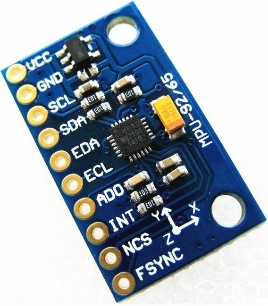
\includegraphics[width=0.2\textwidth]{chapter3/images/mpu9250.jpeg}
    \caption{แสดงเซนเซอร์ IMU MPU9250}
    \label{fig:mpu9250}
\end{figure}

\subsubsection*{Wi-Fi Adapter}
เนื่องจากหน่วยประมวลผลขั้นสูงของหุ่นยนต์ฮิวมานอยด์อุทัยนั้น ไม่สามารถเชื่อมต่อผ่านทาง Wifi ได้
จึงมีตัวรับสัญญาณ Wifi ดังรูปที่ \ref{fig:rpi_wifi_adaptor} ติดตั้งเพิ่มขึ้นมา เพื่อใช้ในการติดต่อสื่อสารระหว่างหน่วยประมวลผลระดับสูงที่ติดตั้งอยู่บนตัวของหุ่นยนต์
และคอมพิวเตอร์ที่เป็นตัวสั่งการซึ่งอยู่นอกตัวของหุ่นยนต์ ซึ่งในงานวิจัยนี้
จะใช้ส่งข้อมูลที่ได้หลังจากการประมวลผลบนคอมพิวเตอร์ไปยังตัวหุ่นยนต์ เช่น การวางแผนการเดิน การคำนวนพลศาสตร์ของหุ่นยนต์
และอื่นๆ โดยการส่งข้อมูลไปยังหน่วยประมวลผลระดับสูงจะมีตัวกลางในการรับส่งสัญญาณ
คือ ตัวกระจายสัญญาณ (Wifi router)\footnote{https://www.alzashop.com/tp-link-archer-c7-d470129.htm}
\begin{figure}[!ht]
    \centering
    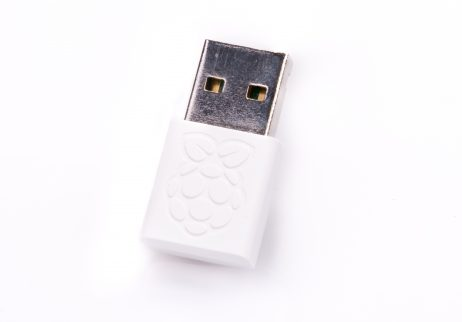
\includegraphics[width=0.3\textwidth]{chapter3/images/rpi_wifi_adaptor.jpg}
    \caption{ตัวรับสัญญาณ Wifi ของ RaspberryPi}
    \label{fig:rpi_wifi_adaptor}
\end{figure}
\begin{figure}[!ht]
    \centering
    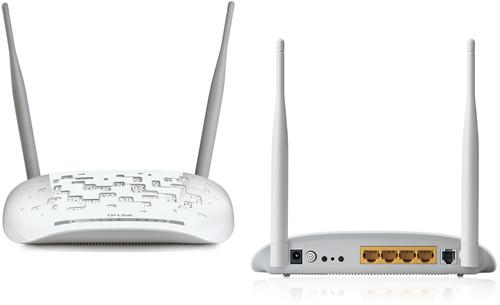
\includegraphics[width=0.3\textwidth]{chapter3/images/wifi_router.jpg}
    \caption{ตัวกระจายและรับส่งสัญญาณ wifi}
    \label{fig:wifi_router}
\end{figure}


\clearpage
\subsubsection*{Ground contact sensor}
เซนเซอร์ตรวจหน้าสัมผัสที่พื้นเป็นเซนเซอร์ที่ถูกติดตั้งบริเวณฝ่าเท้า เพื่อตรวจสอบการเดินของหุ่นยนต์ฮิวมานอยด์ว่าขณะนี้มีการสัมผัสของฝ่าเท้าของหุ่นยนต์กับพื้นหรือไม่ 
ซึ่งในงานวิจัยนี้ได้ใช้หลักการตัวตรวจจับแรงกดแบบค่าความต้านทานหรือ Force Sensing Resistor (FSR)
แนวคิดการออกแบบหลัก คือการออกแบบให้สามารถติดตั้งกับตัวหุ่นยนต์ได้เลย
ใช้ Arduino การพัฒนาซึ่งให้สามารถอ่านค่าได้ทั้งอนาลอคและดิจิตอลได้ อีกทั้งรองรับการต่อเซนเซอร์จำนวน 4 ตัว โดยมีลายวงจรดังรูปที่ \ref{fig:FSR_schematic}
และตัวอย่างของเซนเซอร์ตรวจจับหน้าสัมผัสดังรูป \ref{fig:complete_FSR}
\begin{figure}[!ht]
  \centering
  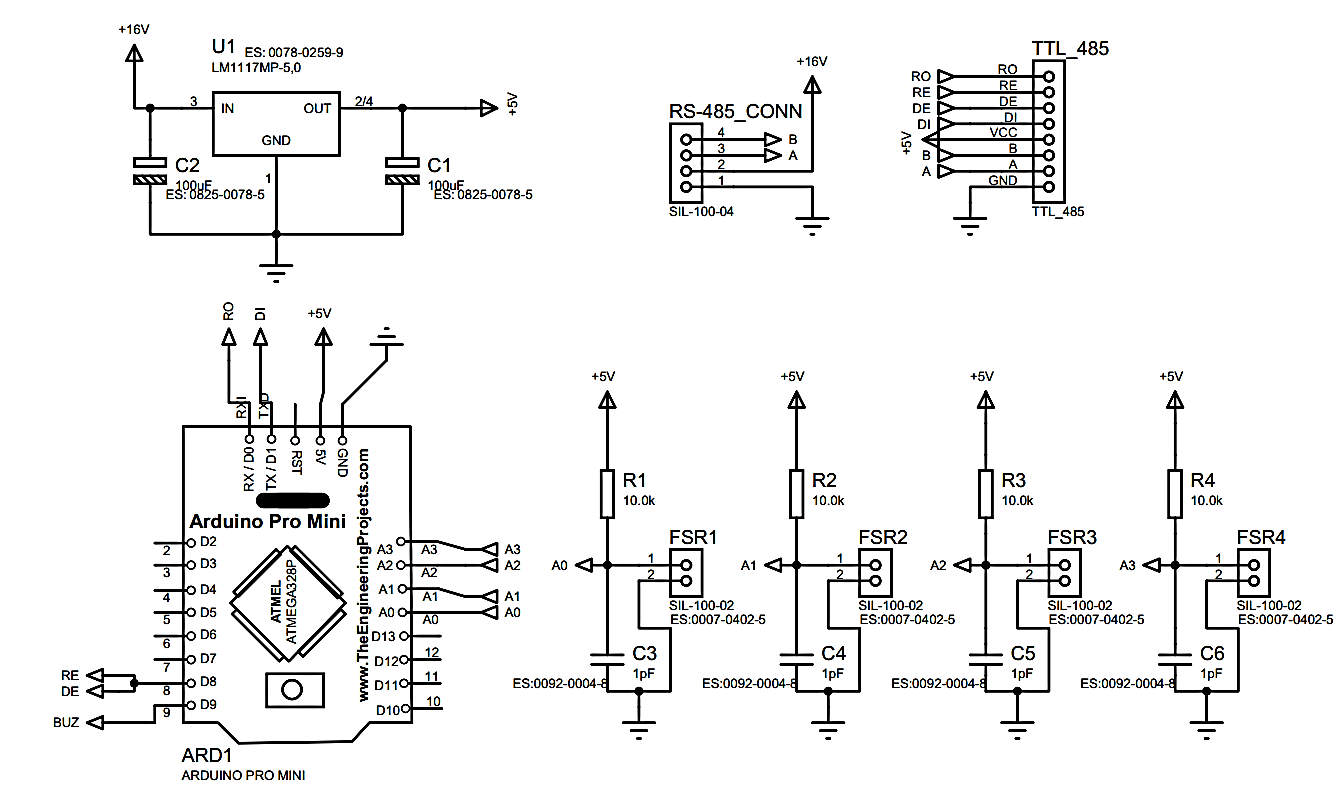
\includegraphics[width=0.8\textwidth]{chapter3/images/FSR_schematic.png}
  \caption{Schematic ของวงจร Ground Contact Sensor}
  \label{fig:FSR_schematic}
\end{figure}

\begin{figure}[!ht]
  \centering
  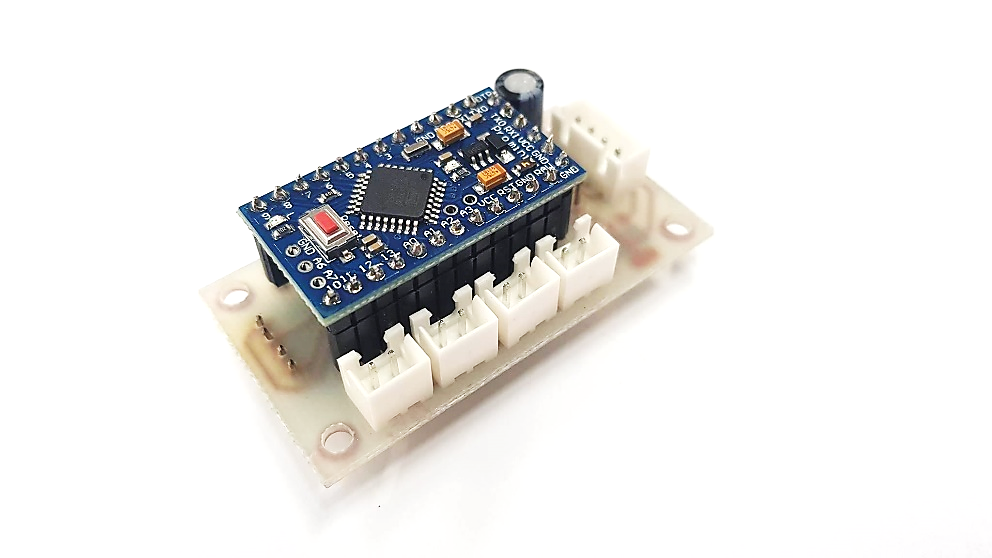
\includegraphics[width=0.8\textwidth]{chapter3/images/complete_FSR.png}
  \caption{แผงวงจร Ground Contact Sensor ที่ประกอบเสร็จแล้ว}
  \label{fig:complete_FSR}
\end{figure}

% \clearpage
% เซนเซอร์ที่เลือกใช้คือ Force Sensitive Resistor (FSR) เป็นเซนเซอร์ที่มีค่าความต้านทานภายในตัวเอง โดยเซนเซอร์นี้มีหลักการทำงานคือ 
% ค่าความต้านทานทางไฟฟ้าของตัวเซนเซอร์จะเปลี่ยนแปลงเมื่อมีแรงเข้ามากระทำกับหน้าสัมผัส เมื่อมีแรงเข้ามากระทำมาก จะทำให้ค่าความต้านทานต่ำ 
% หากไม่มีแรงเข้ามากระทำจะทำให้มีค่าความต้านทานสูง และเมื่อมีการนำเซนเซอร์นี้มาต่อกับตัวต้านทานที่มีค่าคงที่ ในรูปแบบของ Voltage Divider 
% ดังรูปที่ \ref{fig:FSR_schematic} จะทำให้สามารถอ่านค่าแรงดันไฟฟ้าที่เปลี่ยนแปลงตามแรงที่เกิดขึ้นกับหน้าสัมผัสของเซนเซอร์ FSR ได้ 

% \begin{figure}[!ht]
%   \centering
%   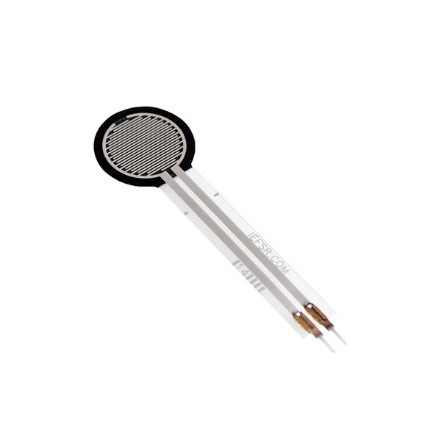
\includegraphics[width=0.3\textwidth]{chapter3/images/FSR.jpg}
%   \caption{Force Sensitive Resistor (FSR) ขนาด 0.5 นิ้ว}
%   \label{fig:FSR}
% \end{figure}

% ข้อดีของ FSR นั้นคือ เป็นเซนเซอร์ที่ถูกพัฒนาและออกแบบมาเพื่อใช้สำหรับการวัดแรงโดยตรง จึงทำให้ใช้งานได้ง่าย และสะดวก ในราคาที่ถูกกว่า 
% เมื่อเทียบกับเซนเซอร์ Load cell ที่มีราคาสูงและการใช้งานจำเป็นที่จะต้องมีวงจรขยายสัญญาณที่ใช้ในการอ่านค่าการบิดของวัสดุจาก 
% แต่ FSR นั้นก็มีข้อเสียเช่นกันคือ ความไม่ทนทานต่อการขีดข่วน เนื่องจากตัวเซนเซอร์ถูกทำมาจากฟิล์มพลาสติกบางๆ ซึ่งหากเกิดการขีดข่วนเกิดขึ้นแล้วอาจทำให้ฟิล์มฉีกขาดได้ 
% หากฟิล์มขาดจะทำให้ค่าความต้านทานออกมาไม่เหมือนเดิม ดังนั้นทางผู้เขียนจึงเลือกที่จะออกแบบโครงครอบสำหรับเซนเซอร์ FSR เพื่อป้องกันจากการถูกขีดข่วนจากภายนอก







%%%%%%%%%%%%%%%%%%%%%%%%%%%%%%%%%%%%%%%%%%%%%%%%%%%%%%%%%%%%%%%%%%%%%%%%%%%%%%%
\clearpage
\subsection{การเชื่อมต่อดิจิตอลเซอร์โวและเซนเซอร์}
โครงสร้างของหุ่นยนต์ฮิวมานอยด์ UTHAI มีขาสองข้างทำให้เกิดองศาอิสระ 12 องศาอิสระ
ผู้วิจัยจึงใช้ดิจิตอลเซอร์โวทั้งหมด 12 ตัว ดิจิตอลเซอร์โวทุกตัวเชื่อมต่อกันแบบสายโซ่เดซี่ (daisy chain) ดังรูปที่ \ref{fig:dynamixel_connect}
ข้างหนึ่งของมอเตอร์ตัวแรกเชื่อมต่อกับแบตเตอร์รี่ 12V และอีกข้างต่อกับ USB2RS485 เพื่อต่อไปยังตัวประมวลผลระดับสูง (Odroid)
และเซนเซอร์หน่วยวัดความเฉื่อย กับเซนเซอร์ตรวจจับหน้าสัมผัสที่พื้นเชื่อมต่อกับตัวประมวลผลระดับต่ำ (Nucleo F411RE)
ดังรูปที่ \ref{fig:odroid2dynamixel}
\begin{figure}[!ht]
    \centering
    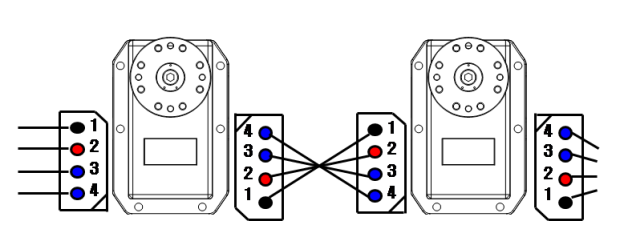
\includegraphics[width=0.8\textwidth]{chapter3/images/dynamixel_connect.png}
    \caption{การเชื่อมต่อกันระหว่างดิจิตอลเซอร์โว}
    \label{fig:dynamixel_connect}
\end{figure}
\begin{figure}[!ht]
    \centering
    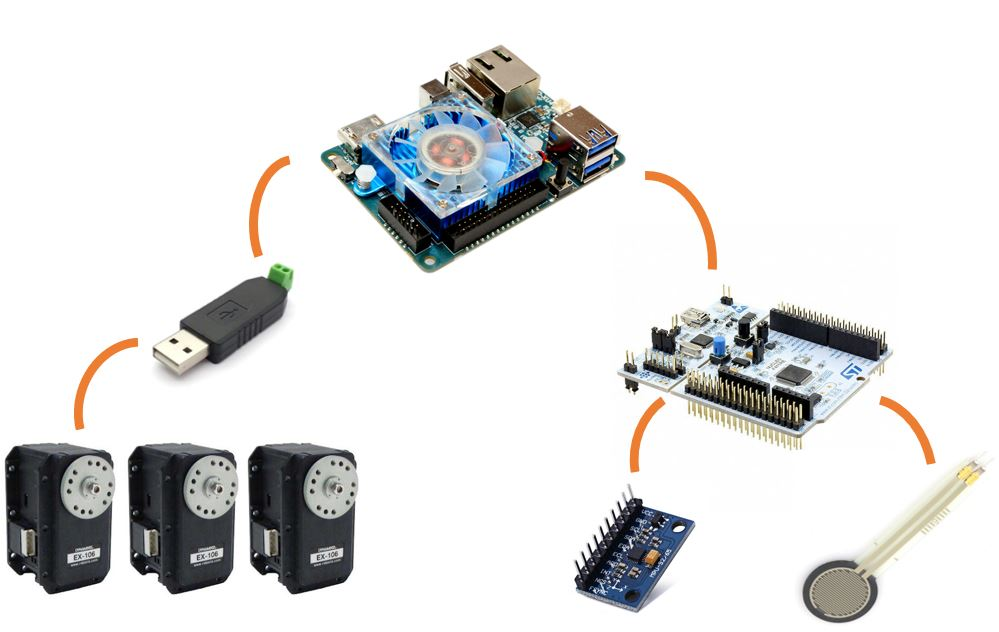
\includegraphics[width=0.9\textwidth]{chapter3/images/odroid2dynamixel.JPG}
    \caption{การเชื่อมต่อระหว่างตัวรับรู้ ตัวประมวลผล และตัวขับเคลื่อน}
    \label{fig:odroid2dynamixel}
\end{figure}


%%%%%%%%%%%%%%%%%%%%%%%%%%%%%%%%%%%%%%%%%%%%%%%%%%%%%%%%%%%%%%%%%%%%%%%%%%%%%%%
\clearpage
\subsection{การตั้งค่าดิจิตอลเซอร์โว}

\begin{wrapfigure}{l}{0.2\textwidth}
    
\includegraphics[width=0.9\linewidth]{chapter3/images/roboplus/roboplus.jpg} 
    \caption*{Roboplus 1.0}
\end{wrapfigure}

ก่อนที่จะเชื่อมต่อดิจิตอลเซอร์โวเข้ากับระบบประมวลผล จำเป็นที่จะต้องมีการตั้งค่า ID, Baudrate, Joint limited 
ของดิจิตอลเซอร์โว โดยการตั้งค่าพารามิเตอร์ของดิจิตอลเซอร์โวนั้น ผู้วิจัยจะใช้โปรแกรมที่มีชื่อว่า
Roboplus 1.0 ซึ่งเป็นเครื่องมือจากบริษัท Robotis ที่จำหน่ายดิจิตอลเซอร์โวนี้ โดยจะช่วยให้สามารถติดต่อกับดิจิตอลเซอร์โว
ตั้งค่าพารามิเตอร์ได้ แต่โปรแกรม Roboplus 1.0 นี้ใช้ได้เฉพาะใน Windows OS เท่านั้น ซึ่งสามารถดาวน์โหลดโปรแกรมได้จากหน้าเว็บไซต์ Robotis\footnote{http://www.robotis.us/roboplus1/}
เมื่อดาวน์โหลดโปรแกรมและติดตั้งเรียบร้อยแล้ว ให้เชื่อมต่อดิจิตอลเซอร์โวกับคอมพิวเตอร์ด้วย USB2RS485
และตั้งค่าพารามิเตอร์โดยทำตามขั้นตอน ดังรูปต่อไปนี้
\begin{figure}[!ht]
    \centering
    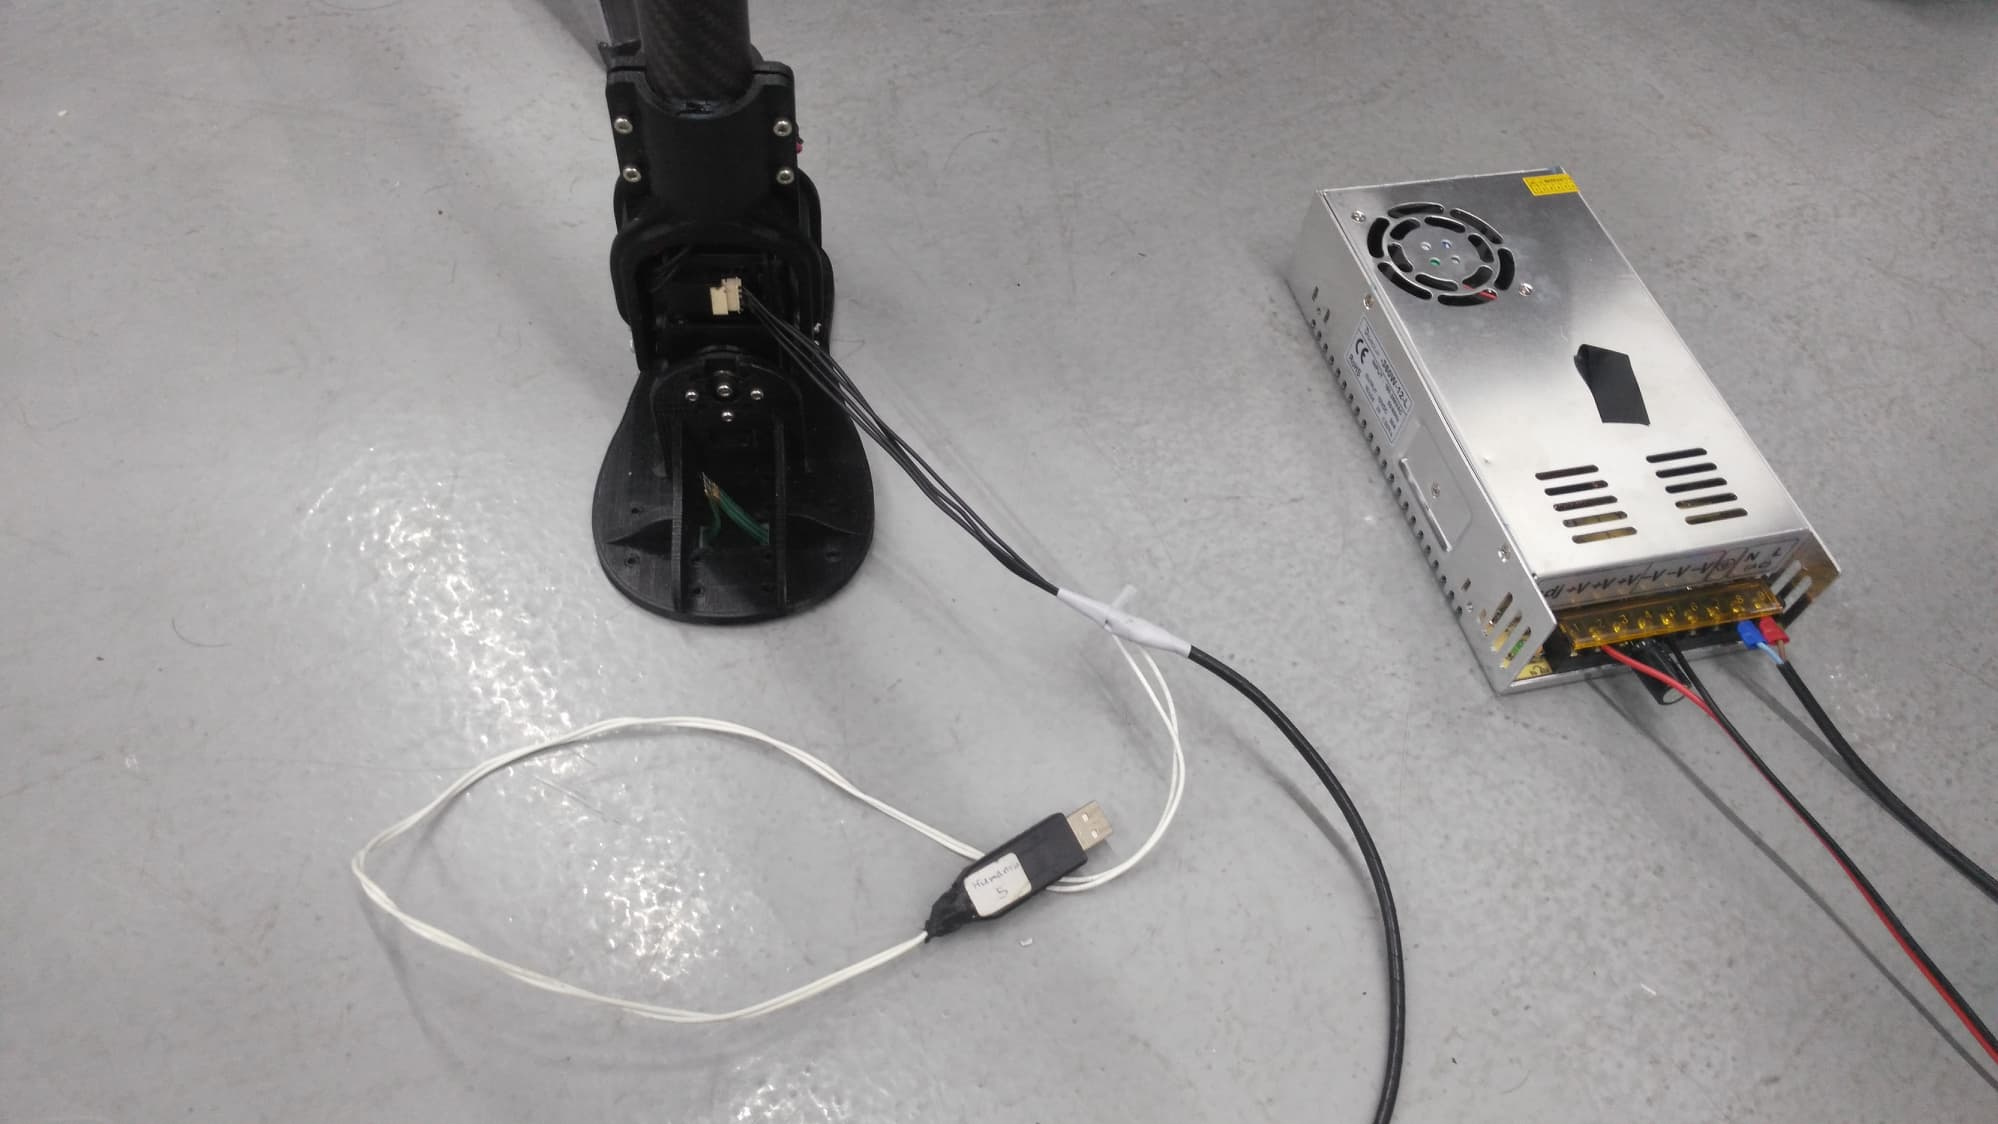
\includegraphics[width=\textwidth]{chapter3/images/roboplus/roboplus0.jpg}
    \caption*{เชื่อมต่อดิจิตอลเซอร์โวเข้ากับคอมพิวเตอร์ด้วย USB2RS485}
\end{figure}
\begin{figure}[!ht]
    \centering
    
\includegraphics[width=0.25\textwidth]{chapter3/images/roboplus/roboplus1.PNG}
    \caption*{เปิดโปรแกรม Roboplus 1.0}
\end{figure}
\begin{figure}[!ht]
    \centering
    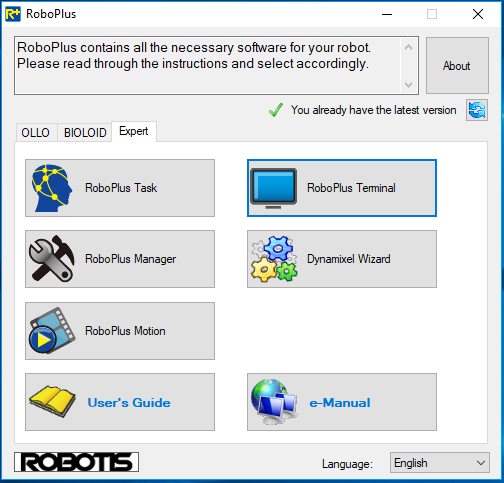
\includegraphics[width=0.55\textwidth]{chapter3/images/roboplus/roboplus2.PNG}
    \caption*{กดเข้าไปที่ Dynamixel Wizard}
\end{figure}
\begin{figure}[!ht]
    \centering
    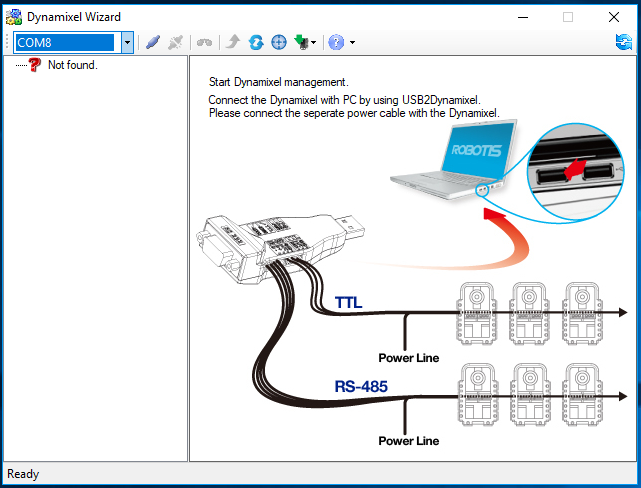
\includegraphics[width=0.55\textwidth]{chapter3/images/roboplus/roboplus3.PNG}
    \caption*{เลือก COM Port ให้ตรงกับ USB2RS485 จากนั้นกด Connect}
\end{figure}
\begin{figure}[!ht]
    \centering
    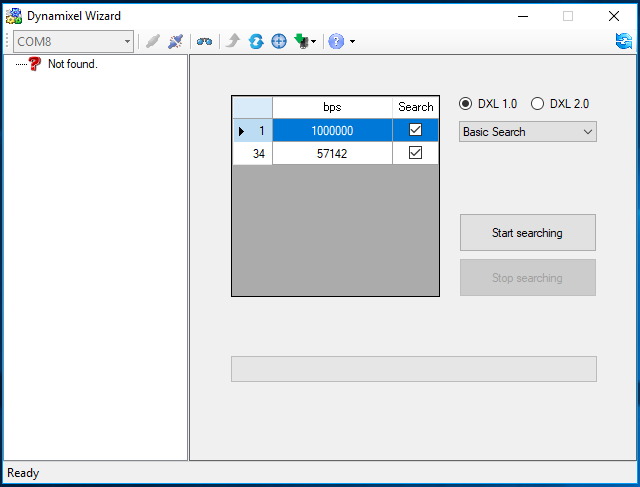
\includegraphics[width=0.55\textwidth]{chapter3/images/roboplus/roboplus4.PNG}
    \caption*{กดเลือกที่ช่อง 1Mbps แล้วกด Start searching}
\end{figure}
\begin{figure}[!ht]
    \centering
    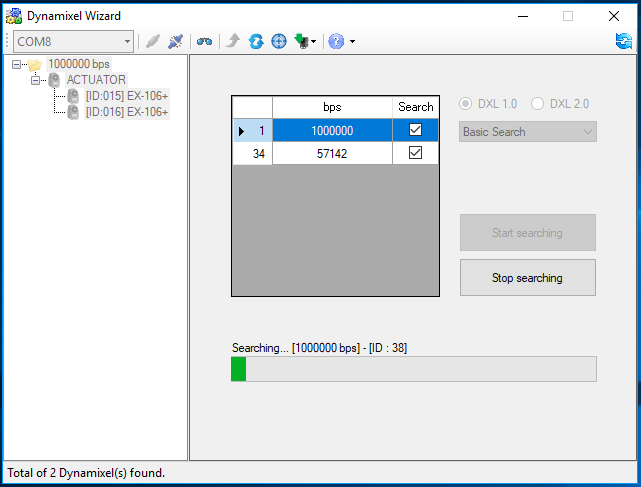
\includegraphics[width=0.55\textwidth]{chapter3/images/roboplus/roboplus5.PNG}
    \caption*{เมื่อเห็นทางด้านซ้ายมือโผล่ ID มอเตอร์ขึ้นมา หากขึ้นแล้วก็สามารถกด Stop Searching ได้}
\end{figure}
\begin{figure}[!ht]
    \centering
    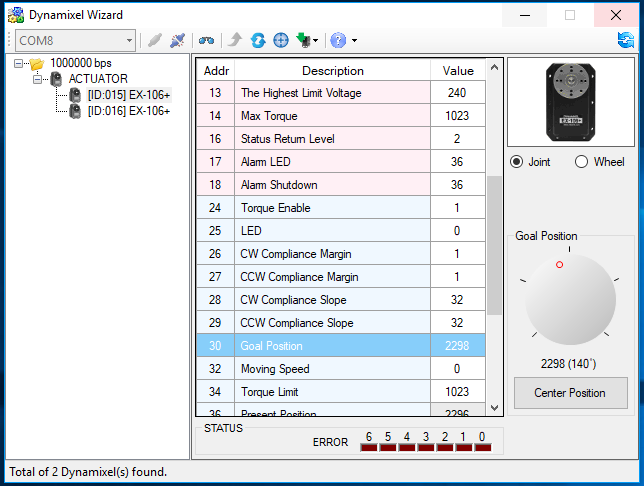
\includegraphics[width=0.55\textwidth]{chapter3/images/roboplus/roboplus6.PNG}
    \caption*{ทดสอบสั่งการมอเตอร์ที่ Addr 30 Goal position ว่าทิศทางถูกต้องหรือไม่}
\end{figure}
\begin{figure}[!ht]
    \centering
    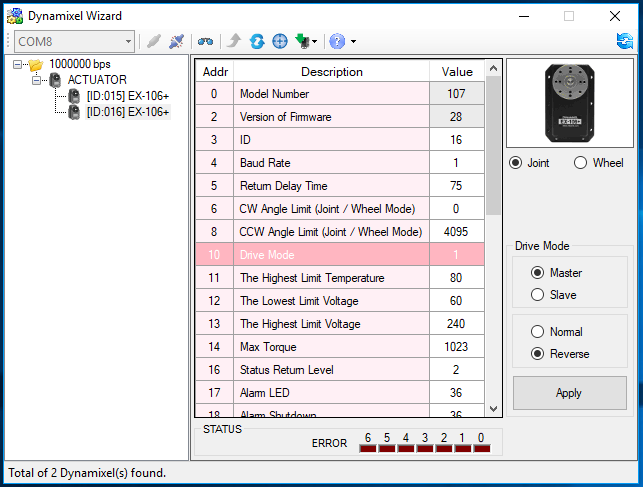
\includegraphics[width=0.55\textwidth]{chapter3/images/roboplus/roboplus7.PNG}
    \caption*{ถ้าทิศทางไม่ถูกต้องสามารถที่จะปรับได้ที่ Addr 10 Drive mode}
\end{figure}

%%%%%%%%%%%%%%%%%%%%%%%%%%%%%%%%%%%%%%%%%%%%%%%%%%%%%%%%%%%%%%%%%%%%%%%%%%%%%%%
\clearpage
\subsection{การเชื่อมต่อหน่วยประมวลผลระดับสูงและระดับต่ำ}
การเชื่อมต่อระหว่างหน่วยประมวลผล นั้นจะเชื่อมต่อกันผ่านสาย USB ชนิด Mini
และส่งข้อมูลหากันผ่าน Serial โดยใช้ rosserial นอกจากจะมีหน่วยประมวลผลแล้วยังมีบอร์ดที่เอาไว้ใช้สำหรับควบคุม
ดิจิตอลเซอร์โวเพื่อเผื่อเอาไว้สำหรับควบคุมการเคลื่อนไหวของแขนหุ่นยนต์ฮิวมานอยด์อุทัย
ดัวรูปที่ \ref{fig:uthai_controller} และทดสอบการสั่งการดังรูปที่ \ref{fig:uthai_drive} 

\begin{figure}[!ht]
    \centering
    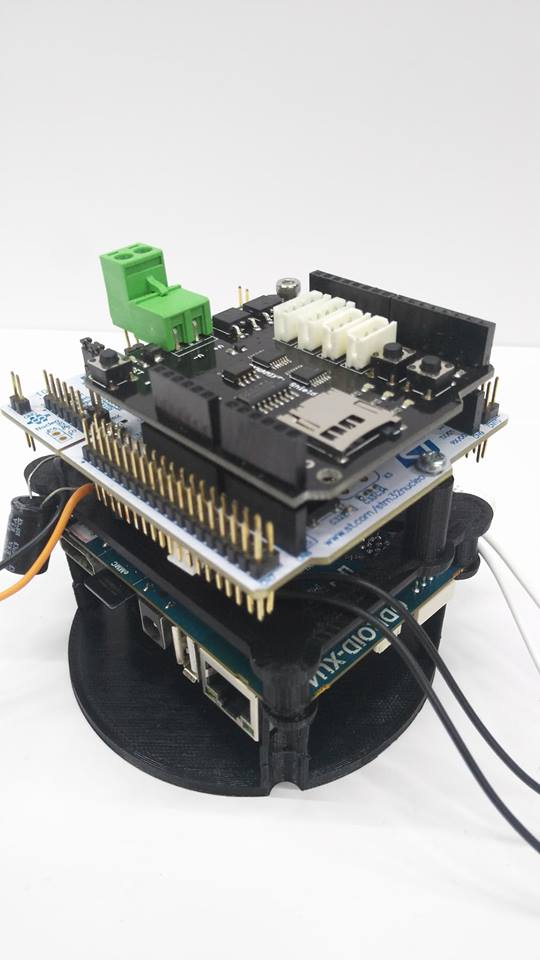
\includegraphics[width=0.4\textwidth]{chapter3/images/uthai_controller.jpg}
    \caption{การเชื่อมต่อกันระหว่างตัวประมวลผล}
    \label{fig:uthai_controller}
\end{figure}

\begin{figure}[!ht]
    \centering
    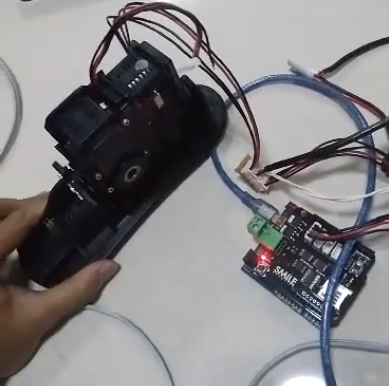
\includegraphics[width=0.5\textwidth]{chapter3/images/clean/uthai_drive.png}
    \caption{ตัวอย่างการใช้งานบอร์ดสั่งการดิจิตอลเซอร์โว}
    \label{fig:uthai_drive}
\end{figure}




